\documentclass[t,ignorenonframetext]{beamer}
%\usepackage{beamerthemeJuanLesPins}%
%\usepackage{beamercolorthemecougar} 
%\usepackage{beamerinnerthemecircles} 
\mode<presentation>
{
  \usetheme{Darmstadt}
  \usecolortheme{rose}
  \usefonttheme{default}
}

%\usefonttheme{structuresmallcapsserif}
\usepackage{enumerate,graphicx,verbatim,url}
\usepackage{fancyvrb}
\usepackage{graphicx}
\usepackage{algorithmic}
\usepackage{caption}
\usepackage{subcaption}


\newcommand\Red[1]{\textcolor{red}{#1}}

\usepackage{tikz}
\usetikzlibrary{arrows,decorations.pathmorphing,fit,positioning}

% The line below is what I talked about that makes all
% items in a list into overlays
%\beamerdefaultoverlayspecification{<+->}

\newcommand{\tc}[1]{$\backslash$\texttt{#1}}
\newcommand{\specialcell}[2][c]{%
  \begin{tabular}[#1]{@{}c@{}}#2\end{tabular}}
  
\title{Lyrics-based Music Genre Analysis using Topic Modelling}
\author{David van Erkelens, Elise Koster \& Sharon Gieske}
\begin{document}
\frame{
\maketitle
}
\frame{
\tableofcontents
}

\section[Introduction]{Introduction}

\subsection{Motivation}
\begin{frame}
\frametitle{Motivation}
~\\
\begin{itemize}
	\item Online music services 
	%\\$\rightarrow$ personalized suggestions based on genre, collective intelligence
	\item Most music classification tasks based on audio signals 
	%\\$\rightarrow$ more storage, more noise-sensitive
	\item Earlier research did not use topic models for genre classification
\end{itemize}
~\\Applications:
\begin{itemize}
\item \textbf{Automatic genre assignment}
\item Finding songs with similar lyrical themes
\item Generation of lyrics
\item Modeling correlation between genres based on topic distributions
\end{itemize}
\end{frame}

\subsection{Project Focus}
\begin{frame}
\frametitle{Project Focus}
~\\~\\
\begin{center}
\Large{Can topic modelling be used for genre modeling based on lyrical themes by extending LDA?}
%\Large{Extension of LDA to genre modeling based on lyrical themes}
\end{center}
~\\~\\
\end{frame}

\section[Approach]{Approach}
\subsection{Framework}

\begin{frame}
\frametitle{Framework}~\\
\begin{enumerate}
	\item Gather dataset using crawler
	\item Preprocessing (removal of stop words etc)
%	\item Gibbs sampling: sample $(topic,word)$ given $p(topic|word)$ and $p(word|topic)$
	\item Model topics and extract topic distribution for documents
%	\item Every genre now has a distribution over topics, and every topic has a distribution over words
	\item Train SVM on array of topic-probabilities per document (and its genre)
	\item Generate `song' of length $n$ for genre $g$: select topic $k \sim \theta_g$ then select word $w \sim \varphi_k$, repeat $n$ times
\end{enumerate}

\end{frame}

\subsection{Methods}
\begin{frame}
\frametitle{Methods}

\textbf{Extension of LDA:}
%\textbf{Latent Dirichlet Allocation:} \\Topic model where each document has a distribution over topics, and each topic has a distribution over words
\begin{columns}
\begin{column}{0.50\textwidth}
	~\\
	\begin{figure}
		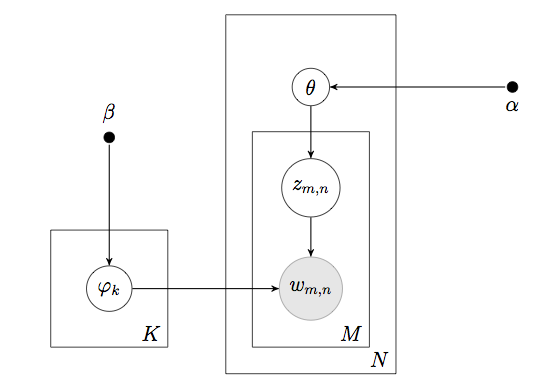
\includegraphics[scale=0.2]{original_lda}
		\caption{Original LDA}
	\end{figure}
\end{column}
\begin{column}{0.50\textwidth}
	\begin{figure}
		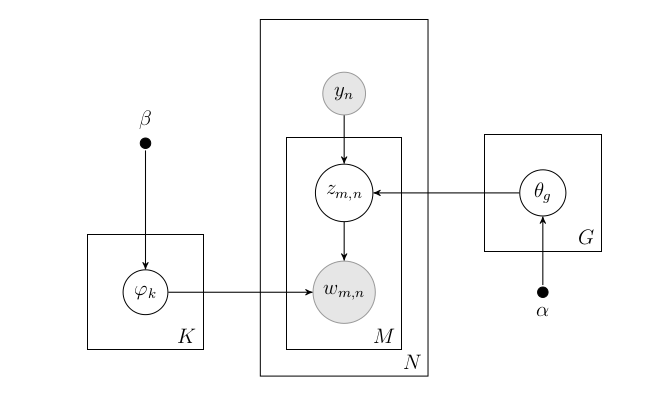
\includegraphics[scale=0.2]{plate2}
		\caption{Extended LDA}
	\end{figure}
\end{column}
\end{columns}
~\\
\textbf{Gibbs sampling:}\\
$P(z_{i,j} = k | Z_{\neg w_{i,j}}, \alpha, \beta, W, Y) \propto \frac{\beta + \widetilde{C}(k, w_{i,j})}{V\beta + \widetilde{C}(k)} \times \frac{\alpha + \widetilde{C}(y_i, k)}{K\alpha + \widetilde{C}(y_i)}$
\end{frame}





\section[Results]{Results}
\subsection{Preliminary Results}
\begin{frame}~\\
\textbf{Topic Modelling}\\
Top topic (defined by its top 20 words) for some genres (after 20 iterations):\\
\begin{table}
\begin{tabular} {|c|l|}
	\hline
	Religious & \specialcell{'lord', 'god', 'praise', 'jesus', 'holy', 'every', 'verse', \\ 'chorus', 'yes', 'glory', 'grace', 'power', 'know', \\'worthy', 'great', 'worship', \\'hallelujah', 'let', 'things', 'spirit'}\\
	\hline
	Holiday & \specialcell{'la', 'star', 'two', 'wish', 'like', 'bring', 'see', 'even', \\'good', 'never', 'new', 'get', 'something', 'moving',\\ 'let', 'sound', 'keep', 'christmas', 'come', 'little'} \\
	\hline 
	Rap & \specialcell{'nigga', 'bh', 'yo', 'got', 'st', 'niz', 'lil', 'get', 'fuck', \\'like', 'shit', 'fuckin', 'hoes', 'homie', 'niggas', \\ 'bang', 'ay', 'fresh', 'friends', 'first'}\\
	\hline
	\end{tabular}
	\caption{Top topics for genres Religious, Holiday and Rap}
	\end{table}
\end{frame}

\begin{frame}
\frametitle{Topic distribution for genres}

\begin{minipage}[b][.35\textheight][t]{.47\textwidth}
\begin{figure}
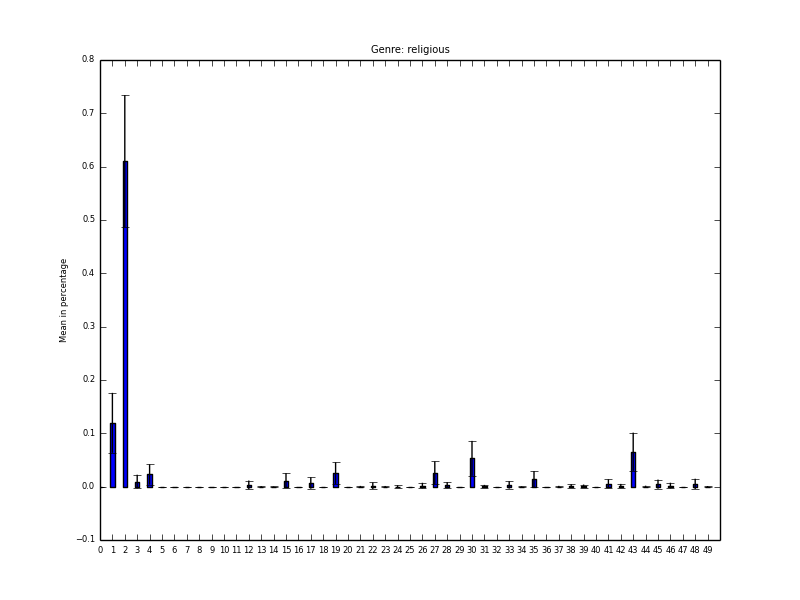
\includegraphics[scale=0.2]{bar_charts/religious}
\caption{Religious}
\end{figure}
\end{minipage}\hfill%
    \begin{minipage}[b][.35\textheight][t]{.47\textwidth}
    \begin{figure}
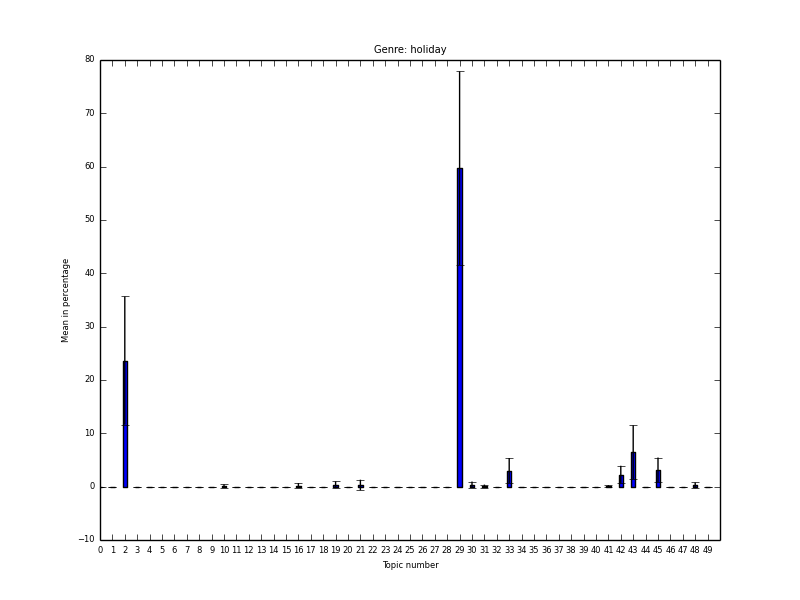
\includegraphics[scale=0.2]{bar_charts/holiday}
\caption{Holiday}
\end{figure}
\end{minipage}\\[2.1em]

   \begin{minipage}[b][.35\textheight][t]{.47\textwidth}
    \begin{figure}
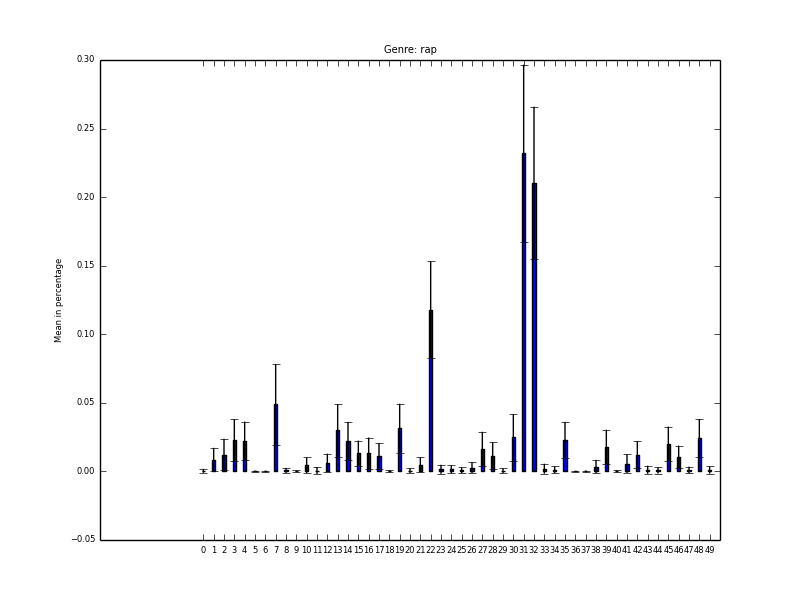
\includegraphics[scale=0.2]{bar_charts/rap}
\caption{Rap}
\end{figure}
\end{minipage}\hfill
    \begin{minipage}[b][.35\textheight][t]{.47\textwidth}
    \begin{figure}
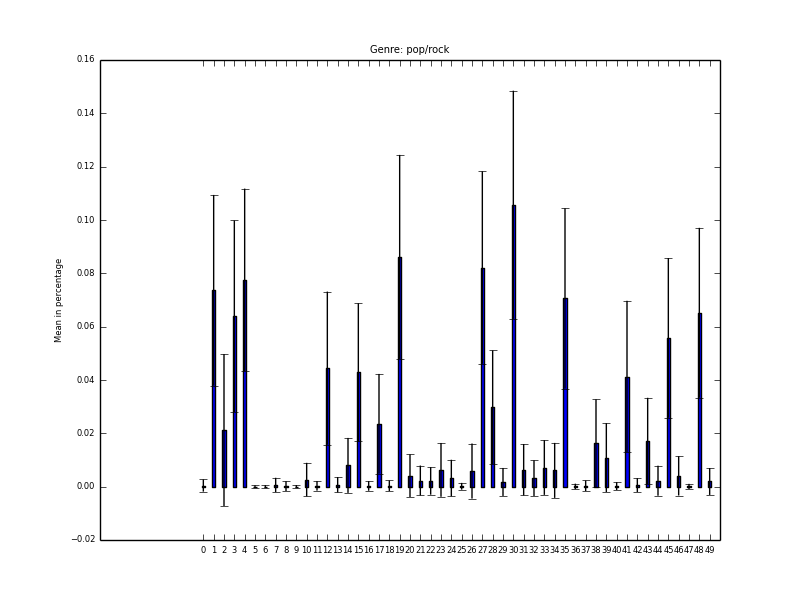
\includegraphics[scale=0.2]{bar_charts/pop-rock}
\caption{Pop/Rock}
\end{figure}
\end{minipage}%
\end{frame}


\begin{frame}
\textbf{Classification}
\begin{itemize}
	\item Baseline classifier: SVM trained on word counts $\sim 47 \%$ correctly classified.
	\item Extended LDA classifier: SVM trained on topic distributions (20 topics, 15 iterations, $\alpha=0.1$, $\beta=0.1$) $\sim 56 \%$ correctly classified
\end{itemize}

\end{frame}

\section{Discussion \& Conclusion}
\begin{frame}~\\
\textbf{Discussion}~\\
\begin{itemize}
%	\item Non-standard topic requires creating own crawler \& preprocessing
	\item Due to many loops, inefficient programming will cost you
	%If you re-compute all word counts every time you go over one word in one document, you're gonna have a (long) bad time. (one iteration of Gibbs sampling took more than 3 days..)
	%\item Sometimes you think you've improved something, but in reality you just broke it (results went from sensible $\rightarrow$ meaningless, turns out we just printed the wrong things)
	%\item LDA is quite a cool algorithm, if you implement it correctly
	\item `Love' is quite a common word in many music genres. So are the words `chorus', and `verse', but that may have to do with our data pre-processing.
\end{itemize}~\\
\textbf{Conclusions}~\\
\begin{itemize}
\setlength{\itemsep}{10pt}\setlength{\itemsep}{5pt}
\item Extended LDA with Gibbs sampling assigns sensible topics to documents
\item Classification using this generative model shows improvement but does not perform optimally. However, more extensive Gibbs sampling is required 

\end{itemize}
\end{frame}

\section[Questions]{Questions}
\begin{frame}
~ \\~ \\~ \\ ~ \\~ \\
\begin{center}\Huge Questions? \end{center} 
\end{frame}


\end{document}